
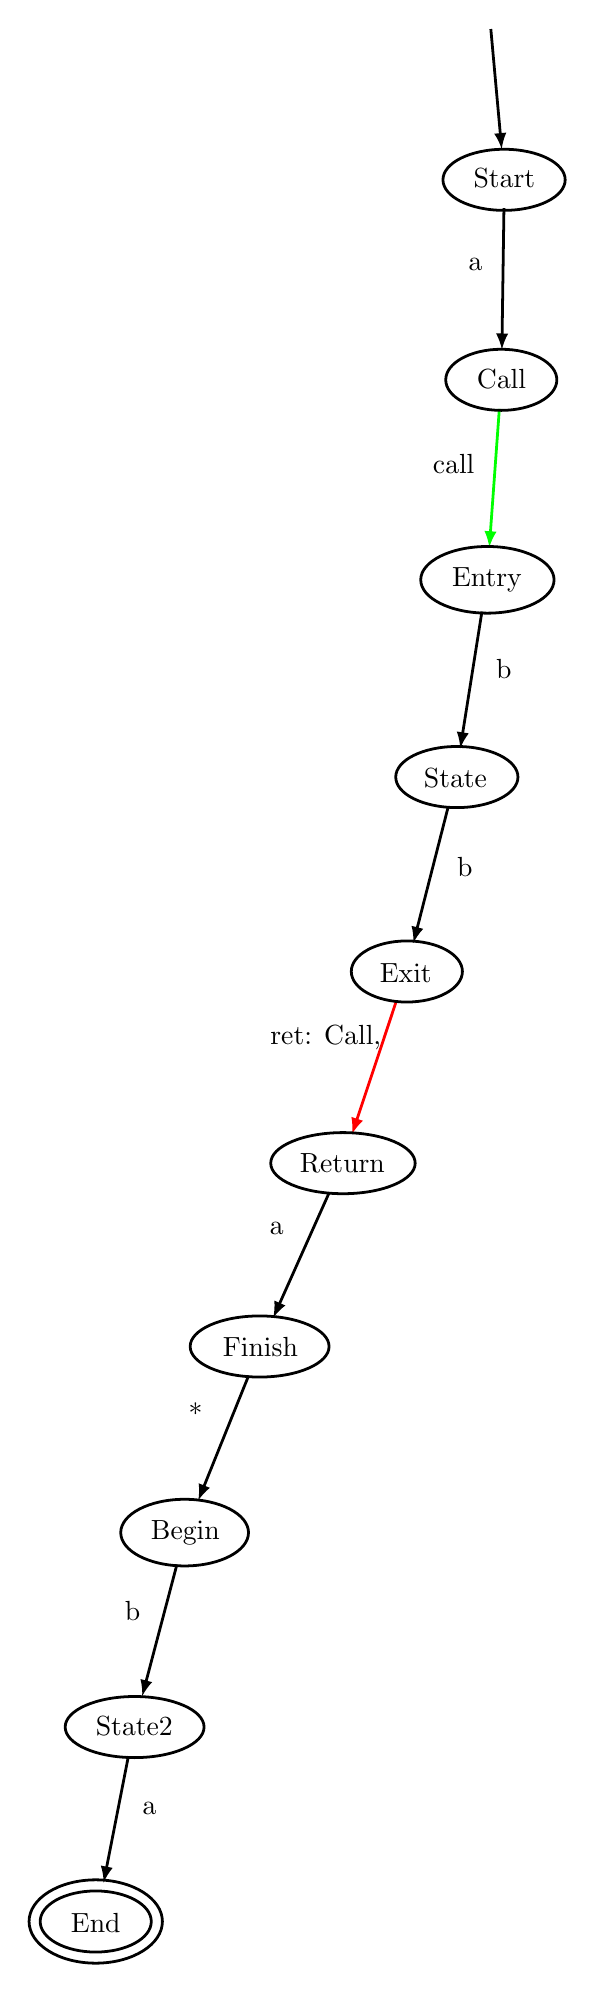
\begin{tikzpicture}[>=latex,line join=bevel,]
  \pgfsetlinewidth{1bp}
%%
\pgfsetcolor{black}
  % Edge: Finish -> Begin
  \draw [->] (80.058bp,212.55bp) .. controls (76.248bp,203.11bp) and (70.527bp,188.93bp)  .. (61.91bp,167.57bp);
  \definecolor{strokecol}{rgb}{0.0,0.0,0.0};
  \pgfsetstrokecolor{strokecol}
  \draw (60.914bp,198.84bp) node {*};
  % Edge: Call -> Entry
  \pgfsetcolor{green}
  \draw [->] (170.3bp,560.53bp) .. controls (169.54bp,550.12bp) and (168.38bp,533.97bp)  .. (166.69bp,510.69bp);
  \definecolor{strokecol}{rgb}{0.0,0.0,0.0};
  \pgfsetstrokecolor{strokecol}
  \draw (153.86bp,540.68bp) node {call};
  % Edge: Entry -> State
  \draw [->] (164.03bp,487.57bp) .. controls (162.37bp,477.07bp) and (159.87bp,461.29bp)  .. (156.23bp,438.34bp);
  \draw (171.94bp,467.06bp) node {b};
  % Edge: Start -> Call
  \draw [->] (171.96bp,632.8bp) .. controls (171.8bp,622.12bp) and (171.56bp,605.41bp)  .. (171.22bp,581.88bp);
  \draw (161.66bp,612.44bp) node {a};
  % Edge: State2 -> End
  \draw [->] (36.761bp,75.521bp) .. controls (34.921bp,66.131bp) and (32.18bp,52.144bp)  .. (27.849bp,30.039bp);
  \draw (44.284bp,56.778bp) node {a};
  % Edge: Return -> Finish
  \draw [->] (109.04bp,278.37bp) .. controls (104.76bp,268.79bp) and (98.344bp,254.45bp)  .. (88.91bp,233.36bp);
  \draw (90.08bp,265.56bp) node {a};
  % Edge: Exit -> Return
  \pgfsetcolor{red}
  \draw [->] (133.14bp,347.12bp) .. controls (129.79bp,337.05bp) and (124.62bp,321.53bp)  .. (117.28bp,299.47bp);
  \definecolor{strokecol}{rgb}{0.0,0.0,0.0};
  \pgfsetstrokecolor{strokecol}
  \draw (107.81bp,334.09bp) node {ret: Call, };
  % Edge: State -> Exit
  \draw [->] (151.8bp,416.95bp) .. controls (149.17bp,406.66bp) and (145.12bp,390.81bp)  .. (139.36bp,368.28bp);
  \draw (157.83bp,395.5bp) node {b};
  % Edge: Begin -> State2
  \draw [->] (54.228bp,144.53bp) .. controls (51.544bp,134.35bp) and (47.565bp,119.26bp)  .. (41.728bp,97.122bp);
  \draw (38.279bp,127.76bp) node {b};
  % Edge: Start__precursor__ -> Start
  \draw [->] (167.23bp,697.28bp) .. controls (168.14bp,687.25bp) and (169.27bp,674.74bp)  .. (171.15bp,654.03bp);
  % Node: Begin
\begin{scope}
  \definecolor{strokecol}{rgb}{0.0,0.0,0.0};
  \pgfsetstrokecolor{strokecol}
  \draw (57bp,156bp) ellipse (23bp and 12bp);
  \draw (57.267bp,156.06bp) node {Begin};
\end{scope}
  % Node: Finish
\begin{scope}
  \definecolor{strokecol}{rgb}{0.0,0.0,0.0};
  \pgfsetstrokecolor{strokecol}
  \draw (84bp,223bp) ellipse (25bp and 11bp);
  \draw (84.279bp,223.01bp) node {Finish};
\end{scope}
  % Node: End
\begin{scope}
  \definecolor{strokecol}{rgb}{0.0,0.0,0.0};
  \pgfsetstrokecolor{strokecol}
  \draw (25bp,16bp) ellipse (20bp and 11bp);
  \draw (25bp,16bp) ellipse (24bp and 15bp);
  \draw (25bp,15.5bp) node {End};
\end{scope}
  % Node: Exit
\begin{scope}
  \definecolor{strokecol}{rgb}{0.0,0.0,0.0};
  \pgfsetstrokecolor{strokecol}
  \draw (137bp,358bp) ellipse (20bp and 11bp);
  \draw (136.61bp,357.54bp) node {Exit};
\end{scope}
  % Node: State2
\begin{scope}
  \definecolor{strokecol}{rgb}{0.0,0.0,0.0};
  \pgfsetstrokecolor{strokecol}
  \draw (39bp,86bp) ellipse (25bp and 11bp);
  \draw (38.867bp,86.27bp) node {State2};
\end{scope}
  % Node: Return
\begin{scope}
  \definecolor{strokecol}{rgb}{0.0,0.0,0.0};
  \pgfsetstrokecolor{strokecol}
  \draw (114bp,289bp) ellipse (26bp and 11bp);
  \draw (113.78bp,288.96bp) node {Return};
\end{scope}
  % Node: Start
\begin{scope}
  \definecolor{strokecol}{rgb}{0.0,0.0,0.0};
  \pgfsetstrokecolor{strokecol}
  \draw (172bp,643bp) ellipse (22bp and 11bp);
  \draw (172.11bp,643.47bp) node {Start};
\end{scope}
  % Node: State
\begin{scope}
  \definecolor{strokecol}{rgb}{0.0,0.0,0.0};
  \pgfsetstrokecolor{strokecol}
  \draw (155bp,428bp) ellipse (22bp and 11bp);
  \draw (154.52bp,427.59bp) node {State};
\end{scope}
  % Node: Call
\begin{scope}
  \definecolor{strokecol}{rgb}{0.0,0.0,0.0};
  \pgfsetstrokecolor{strokecol}
  \draw (171bp,571bp) ellipse (20bp and 11bp);
  \draw (171.07bp,571.17bp) node {Call};
\end{scope}
  % Node: Entry
\begin{scope}
  \definecolor{strokecol}{rgb}{0.0,0.0,0.0};
  \pgfsetstrokecolor{strokecol}
  \draw (166bp,499bp) ellipse (24bp and 12bp);
  \draw (165.85bp,499.05bp) node {Entry};
\end{scope}
%
\end{tikzpicture}
